\chapter{संरक्षण जीवविज्ञान}\label{ch:b3:conservation-biology}

1813 में ऑडुबन ने केंटकी के ऊपर से यात्री कबूतरों का कोई झुंड तीन दिन
तक गुज़रते देखा, जो आकाश को अँधेरा कर रहा था; वे शायद पाँच अरब रहे
होंगे, उत्तरी अमेरिका के सारे पक्षियों का चौथाई। 1~सितंबर 1914 को उनमें
से आख़िरी, मार्था नाम की कोई मादा, सिनसिनाटी चिड़ियाघर में मर गई। जब उस
जाति का ह्रास शुरू हुआ तब वह दुर्लभ नहीं थी; उसे रेलगाड़ी भर-भर कर काटा
जाता था, और उसके वन काटे जा रहे थे, और जो पक्षी केवल विशाल बस्तियों में
प्रजनन करता था वह उन बस्तियों के किसी ऐसे आकार से नीचे विरल हो जाने पर
प्रजनन कर ही नहीं सका जिसे किसी ने मापा नहीं था। 1995 में न्यूज़ीलैंड का
उड़ानहीन निशाचर तोता काकापो इक्यावन पक्षियों तक घट गया था; तब से हर एक
का नाम रखा गया है, तौल हुई है, प्रेषित्र लगा है और, ठीक क्षण पर, कोई
अतिरिक्त भोजन दिया गया है, और अब ढाई सौ हैं। उसी वर्ष इकतीस भूरे भेड़िये
येलोस्टोन में छोड़े गए, आख़िरी देशज झुंड के मारे जाने के सत्तर वर्ष बाद;
दो दशकों के भीतर एल्क हट गए, नदियों के किनारे विलो लौट आए, और उनके साथ
बीवर भी। संरक्षण जीवविज्ञान इस पुस्तक की समष्टि आनुवंशिकी, पारिस्थितिकी
तथा व्यवहार का किसी एक व्यावहारिक प्रश्न पर अनुप्रयोग है --- जातियों को
लुप्त होने से कैसे बचाया जाए --- और उसका अंकगणित छोटी संख्याओं का
अंकगणित है।

\section{छोटी समष्टियाँ क्यों मर जाती हैं}

\begin{definition}[छोटेपन के जोखिम]\label{def:b3:conservation-biology:small}
\index{जनसांख्यिकीय प्रसंभाव्यता}\index{पर्यावरणीय प्रसंभाव्यता}\index{ऐली प्रभाव}\index{विलोपन भँवर}\index{न्यूनतम व्यवहार्य समष्टि}
कोई बड़ी समष्टि तब घटती है जब उसकी मृत्यु-दर उसकी जन्म-दर से बढ़ जाए;
कोई छोटी समष्टि दोनों में किसी बदलाव के बिना ही मिट सकती है।
\emph{जनसांख्यिकीय प्रसंभाव्यता} वह संयोग है कि थोड़े-से व्यष्टियों में
जन्म लेने वालों से अधिक मर जाएँ, या सारे बचे हुए नर ही हों: वह कुछ दर्जन
से नीचे मायने रखती है। \emph{पर्यावरणीय प्रसंभाव्यता} --- कोई बुरी
सर्दी, कोई सूखा, कोई रोग --- हर व्यष्टि पर एक साथ पड़ती है, और कुछ सौ की
कोई समष्टि, जिसे कोई बड़ी समष्टि झेल जाती, मिटाई जा सकती है;
\emph{महाविपदाएँ} उसकी पुच्छ हैं। \emph{ऐली प्रभाव} प्रति-व्यष्टि
वृद्धि-दर को कम घनत्व पर गिरा देता है --- संगी मिलते नहीं, बस्ती बनाकर
प्रजनन करने वाले घोंसला बना नहीं पाते, झुंड अपने बच्चों की रक्षा नहीं कर
पाते, यात्री कबूतर के झुंड उन परभक्षियों को तृप्त नहीं कर पाए जो उनके
शिशुओं को लेते थे --- ताकि किसी देहली घनत्व से नीचे वह समष्टि अपने आप ही
शून्य की ओर घटती जाए। और कुछ सौ से नीचे, अगले अनुभाग की आनुवंशिक
प्रक्रियाएँ पीढ़ी-दर-पीढ़ी सुयोग्यता घटाती हैं। ये एक-दूसरे को पोसती हैं:
कोई छोटी होती समष्टि विविधता खोती है, कम उर्वर हो जाती है, और छोटी होती
है, संयोग की मार झेलने की अधिक संभावना रखती है, और अधिक खोती है --- वही
\emph{विलोपन भँवर} (गिलपिन तथा सूले, 1986)। कोई \emph{न्यूनतम व्यवहार्य
समष्टि} वह आकार है जिससे ऊपर किसी कहे हुए क्षितिज पर विलोपन की प्रायिकता
(मान लीजिए किसी शताब्दी में \qty{5}{\%}) स्वीकार्य हो; वह उस जाति के
जीवविज्ञान पर और इस पर निर्भर करती है कि उसका पर्यावरण कितना परिवर्तनशील
है, और प्रायः हज़ारों में होती है।
\end{definition}

\begin{omfigure}
\begin{tikzpicture}[every node/.style={font=\scriptsize}, >=stealth]
  \node[draw, thick, rounded corners, fill=omThm!20, align=center] (small) at (0,0) {समष्टि\\छोटी हो जाती है};
  \node[draw, thick, rounded corners, fill=omDef!20, align=center] (drift) at (3.4,1.6) {अपवाह तथा अंतःप्रजनन:\\विविधता खोई, $F$ बढ़ा};
  \node[draw, thick, rounded corners, fill=omDef!20, align=center] (fit) at (6.8,0) {सुयोग्यता गिरी:\\कम बच्चे, अधिक रोग};
  \node[draw, thick, rounded corners, fill=omDef!20, align=center] (chance) at (3.4,-1.6) {जनसांख्यिकीय तथा पर्यावरणीय\\संयोग अधिक काटते};
  \node[draw, thick, rounded corners, fill=omProp!25, align=center] (allee) at (9.9,0) {ऐली प्रभाव:\\वृद्धि-दर ऋणात्मक};
  \draw[->, very thick] (small) -- (drift); \draw[->, very thick] (drift) -- (fit); \draw[->, very thick] (fit) -- (chance); \draw[->, very thick] (chance) -- (small);
  \draw[->, thick, omProp!80!black] (fit) -- (allee); \draw[->, thick, omProp!80!black] (allee.south) .. controls (9.9,-3) and (0,-3.4) .. (small.south);
  \node[align=center, font=\tiny] at (3.4,0) {विलोपन भँवर:\\हर चक्कर समष्टि को\\छोटा करता और अगला तेज़ करता};
  \node[left, align=right, font=\tiny] at (-1.7,1.5) {आवास-हानि, कटाई,\\आक्रामक परभक्षी, रोग\\समष्टि को भीतर धकेलते};
  \draw[->, thick, gray] (-1.6,1.2) -- (small.north west);
\end{tikzpicture}

{\small \omterm{def:b3:conservation-biology:small}{विलोपन भँवर}। कोई बाहरी चोट किसी समष्टि को छोटा कर देती है; फिर
छोटापन विविधता खोता है, सुयोग्यता गिराता है, समष्टि को संयोग के सामने खोल
देता है, और उसे और भी छोटा कर देता है। संरक्षण का काम इस फंदे को बंद
होने से पहले तोड़ना है।}
\end{omfigure}

\begin{theorem}[प्रभावी समष्टि आकार]\label{thm:b3:conservation-biology:ne}
\index{प्रभावी समष्टि आकार}\index{लिंग अनुपात}\index{हरात्मक माध्य}\index{अंतःप्रजनन गुणांक}\index{विषमयुग्मजता}
जिस दर से कोई समष्टि विविधता खोती है और अंतःप्रजनन जोड़ती है वह उसके
गणना-आकार $N$ से नहीं बल्कि उसके \emph{प्रभावी आकार} $N_{e}$ से तय होती
है: यानी किसी आदर्श समष्टि का वह आकार --- अचल, यादृच्छिक संगम वाली,
बराबर \omterm{thm:b3:conservation-biology:ne}{लिंग अनुपात} वाली, प्वासों कुल-आकारों वाली --- जो उसी दर से
विषमयुग्मजता खोती। आदर्श से तीन विचलन उसे नीचे लाते हैं। असमान \omterm{thm:b3:conservation-biology:ne}{लिंग
अनुपात}, जिसमें $N_{m}$ प्रजननशील नर और $N_{f}$ मादाएँ हों:
\[
N_{e} = \frac{4N_{m}N_{f}}{N_{m} + N_{f}} ;
\]
एक नर और सौ मादाएँ $N_{e} \approx 4$ देते हैं। $t$ पीढ़ियों भर
उतार-चढ़ाव वाला आकार: $N_{e}$ उन पीढ़ी-आकारों का \emph{\omterm{thm:b3:conservation-biology:ne}{हरात्मक माध्य}}
है, $1/N_{e} = (1/t)\sum 1/N_{i}$, जिस पर सबसे छोटा हावी रहता है ---
हज़ार की कोई समष्टि जो एक बार दस से गुज़री हो उस अवधि भर $N_{e}$ सौ के
पास रखती है। और प्वासों से ऊपर कुल-आकार का प्रसरण उसे और नीचे लाता है।
प्रभावी आकार $N_{e}$ की किसी समष्टि में \emph{\omterm{thm:b3:conservation-biology:ne}{अंतःप्रजनन गुणांक}} $F$ ---
यानी वह प्रायिकता कि किसी व्यष्टि में किसी स्थल के दोनों युग्मविकल्पी
किसी एक पुरखा युग्मविकल्पी की प्रतियाँ हों --- प्रति पीढ़ी $1/2N_{e}$ से
बढ़ता है,
\[
F_{t} = 1 - \Bigl(1 - \frac{1}{2N_{e}}\Bigr)^{t} \approx \frac{t}{2N_{e}},
\qquad H_{t} = H_{0}\Bigl(1 - \frac{1}{2N_{e}}\Bigr)^{t} ,
\]
और \emph{विषमयुग्मजता} $H$ उसी दर से क्षीण होती है। फ़्रैंकलिन का
अँगूठा-नियम, ``50/500'': $N_{e} \ge 50$ अंतःप्रजनन को प्रति पीढ़ी
\qty{1}{\%} से नीचे रखता है, यानी वह दर जो पशु-प्रजनक सह लेते हैं; $N_{e} \ge
500$ उत्परिवर्तन को वह विविधता बदल देने देता है जो अपवाह हटाता है। चूँकि $N_{e}$
प्रायः गणना-आकार का दसवाँ भाग होता है, यह नियम पाँच सौ से पाँच हज़ार की
समष्टियाँ माँगता है।
\end{theorem}
\begin{proof}
समष्टि से यादृच्छिक खींचे गए दो युग्मक आदर्श समष्टि में $1/2N$ प्रायिकता
से एक ही जनकीय युग्मविकल्पी की प्रतियाँ होते हैं, और वही $F$ की वृद्धि
है; विषमयुग्मजता $1 - F$ के अनुपात में है, इसलिए हर पीढ़ी उसे
$(1 - 1/2N_{e})$ से गुणा करती है, जिससे वह चरघातांकी क्षय मिलता है और,
$t \ll N_{e}$ के लिए, $F$ की रैखिक वृद्धि। \omterm{thm:b3:conservation-biology:ne}{लिंग अनुपात}: आधे जीन हर लिंग
से आते हैं, इसलिए दो युग्मकों के किसी जनकीय युग्मविकल्पी को साझा करने की
संभावना $\tfrac{1}{4}\cdot\tfrac{1}{2N_{m}} +
\tfrac{1}{4}\cdot\tfrac{1}{2N_{f}}$ है (युग्मों का चौथाई भाग दोनों
पैतृक, चौथाई दोनों मातृक); इसे $1/2N_{e}$ के बराबर रखने पर
$1/N_{e} = 1/(4N_{m}) + 1/(4N_{f})$ मिलता है, यानी वही सूत्र।
उतार-चढ़ाव: $t$ पीढ़ियों बाद विषमयुग्मजता $H_{0}\prod(1 - 1/2N_{i})
\approx H_{0}\exp(-\sum 1/2N_{i})$ है, जो $H_{0}\exp(-t/2N_{e})$ के
बराबर है जब $1/N_{e}$ उन $1/N_{i}$ का औसत हो। अंतःप्रजनन सुयोग्यता गिराता
है क्योंकि वह अप्रभावी हानिकारक युग्मविकल्पियों को समयुग्मज के रूप में
उघाड़ देता है --- यानी \emph{अंतःप्रजनन अवसाद}, अधिकांश बहिःप्रजनी
जातियों में $F$ के हर \qty{10}{\%} पर उत्तरजीविता या जननक्षमता में कुछ
प्रतिशत की गिरावट।
\end{proof}

\begin{omfigure}
\begin{tikzpicture}
\begin{axis}[
  width=0.46\linewidth, height=5.2cm,
  axis x line=bottom, axis y line=left,
  xmin=0, xmax=1, ymin=0, ymax=1.05,
  xlabel={प्रजननशीलों का वह अंश जो नर है}, ylabel={$N_{e}/N$},
  xlabel style={font=\small, at={(axis description cs:0.5,-0.12)}, anchor=north}, ylabel style={font=\small},
  tick label style={font=\small}, xtick={0,0.1,0.5,0.9,1}, ytick={0.36,1},
  clip=false,
]
\addplot[very thick, omDef, domain=0.005:0.995, samples=100] {4*x*(1-x)};
\draw[dashed, gray] (axis cs:0.1,0) -- (axis cs:0.1,0.36) -- (axis cs:0,0.36);
\node[font=\scriptsize, omDef, anchor=south] at (axis cs:0.5,1.0) {बराबर लिंग: $N_{e} = N$};
\node[font=\scriptsize, anchor=west, align=left] at (axis cs:0.12,0.2) {दस में एक नर\\प्रजननशील: $N_{e} = 0.36N$};
\end{axis}
\begin{axis}[
  at={(0.5\linewidth,0)}, anchor=south west,
  width=0.46\linewidth, height=5.2cm,
  axis x line=bottom, axis y line=left,
  xmin=0, xmax=100, ymin=0, ymax=1.05,
  xlabel={पीढ़ियाँ}, ylabel={विषमयुग्मजता $H_{t}/H_{0}$},
  xlabel style={font=\small, at={(axis description cs:0.5,-0.12)}, anchor=north}, ylabel style={font=\small},
  tick label style={font=\small}, xtick={0,25,50,75,100}, ytick={0.37,0.6,0.9,1},
  yticklabels={0.37,0.6,0.9,1},
  clip=false,
]
\addplot[very thick, omThm, domain=0:100, samples=60] {(1-1/20)^x};
\addplot[very thick, omMeth!70!black, domain=0:100, samples=60] {(1-1/100)^x};
\addplot[very thick, omDef, domain=0:100, samples=60] {(1-1/1000)^x};
\node[font=\scriptsize, omThm, anchor=north west] at (axis cs:12,0.55) {$N_{e} = 10$};
\node[font=\scriptsize, omMeth!70!black, anchor=south west] at (axis cs:50,0.62) {$N_{e} = 50$};
\node[font=\scriptsize, omDef, anchor=south west] at (axis cs:60,0.95) {$N_{e} = 500$};
\end{axis}
\end{tikzpicture}

{\small बाएँ: कोई तिरछा \omterm{thm:b3:conservation-biology:ne}{लिंग अनुपात} प्रभावी आकार को कैसे छोटा करता है ---
जिस हरम-जाति में नरों का दसवाँ भाग ही प्रजनन करे उसका $N_{e}$ उसकी गणना
का तिहाई होता है। दाएँ: विषमयुग्मजता प्रति पीढ़ी $(1 - 1/2N_{e})$ से
क्षीण होती हुई --- दस की कोई समष्टि किसी शताब्दी में अपनी अधिकांश
विविधता खो देती है, पाँच सौ की लगभग कुछ भी नहीं।}
\end{omfigure}

\begin{proof}[प्रमाण-सामग्री]
फ़्लोरिडा पैंथर, जो 1990 के दशक में कोई पच्चीस प्राणियों तक घट गया था,
मुड़ी हुई पूँछें, अनवतरित वृषण, हृदय-दोष और ऐसे शुक्राणु दिखाता था
जिनमें \qty{90}{\%} असामान्य थे --- यानी दिखता हुआ अंतःप्रजनन अवसाद;
1995 में टेक्सस से लाई गई आठ मादाओं (\emph{आनुवंशिक बचाव}) ने उस समष्टि
को तिगुना कर दिया और वे दोष पीछे हट गए। आइल रॉयल के भेड़िये, जिन्हें
1949 में किसी एक जोड़े ने बसाया था और जो अलग-थलग रहे, 2018 तक दो अत्यंत
अंतःप्रजनित व्यष्टियों तक घट गए, और जाँचे गए अधिकांश कंकालों में
मेरुदंडीय विकृतियाँ थीं। इलिनॉय का बड़ा प्रेयरी मुर्ग़ा हज़ारों से पचास
तक गिरा, और उसके अंडों की स्फुटन-दर \qty{93}{\%} से \qty{56}{\%} तक, और
दूसरे राज्यों से पक्षी लाए जाने के बाद उसने वापसी की। संग्रहालयी खालों
तथा प्राचीन DNA ने हर मामले में विषमयुग्मजता की हानि को ह्रास-पूर्व
समष्टि के सामने सीधे मापने दिया।
\end{proof}

\begin{omfigure}
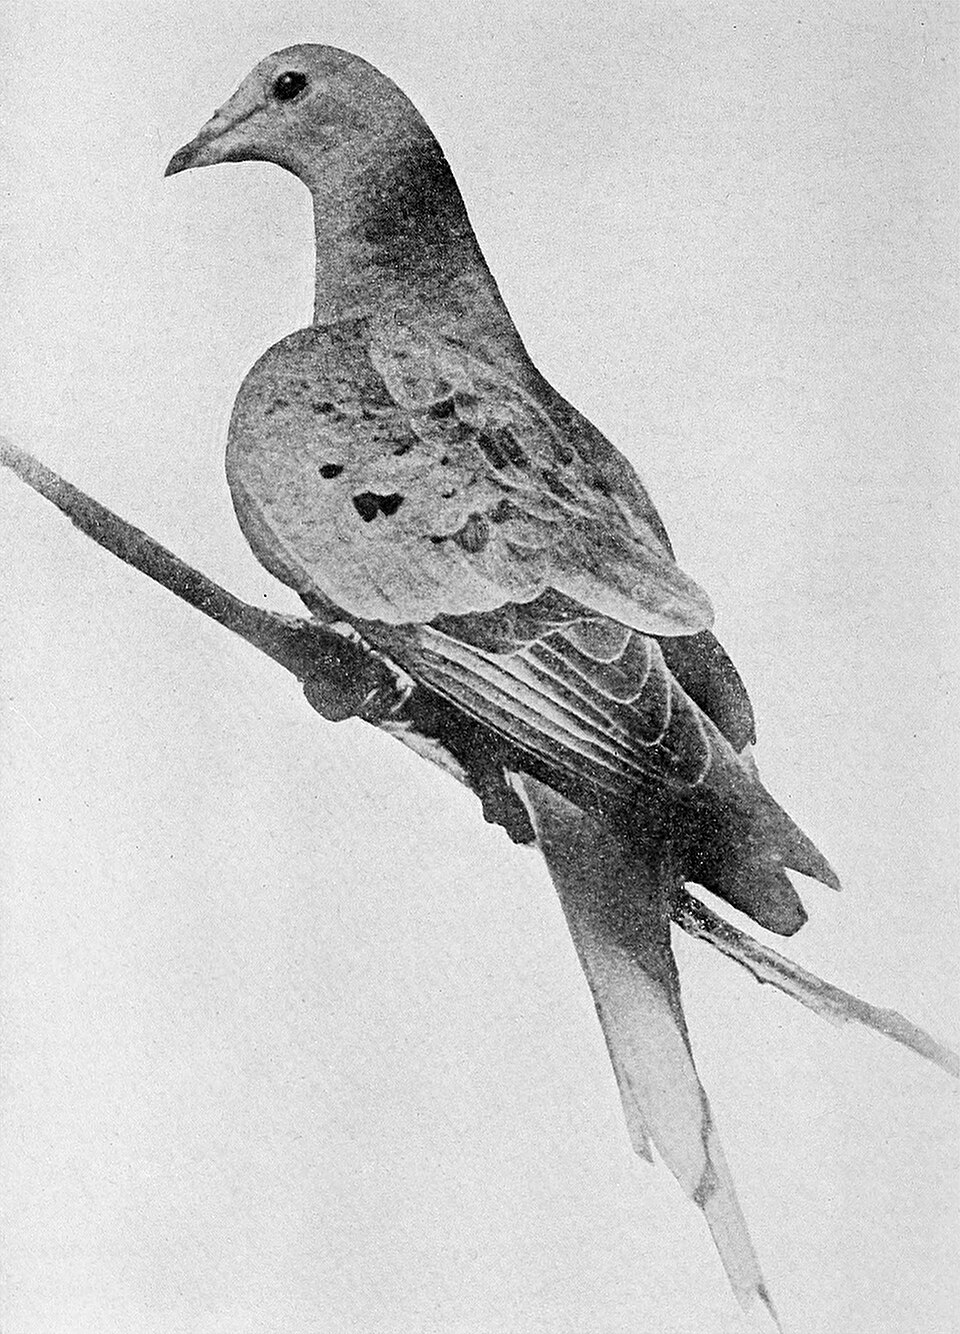
\includegraphics[width=0.4\linewidth]{images/book5/martha.jpg}\hspace{0.04\linewidth}
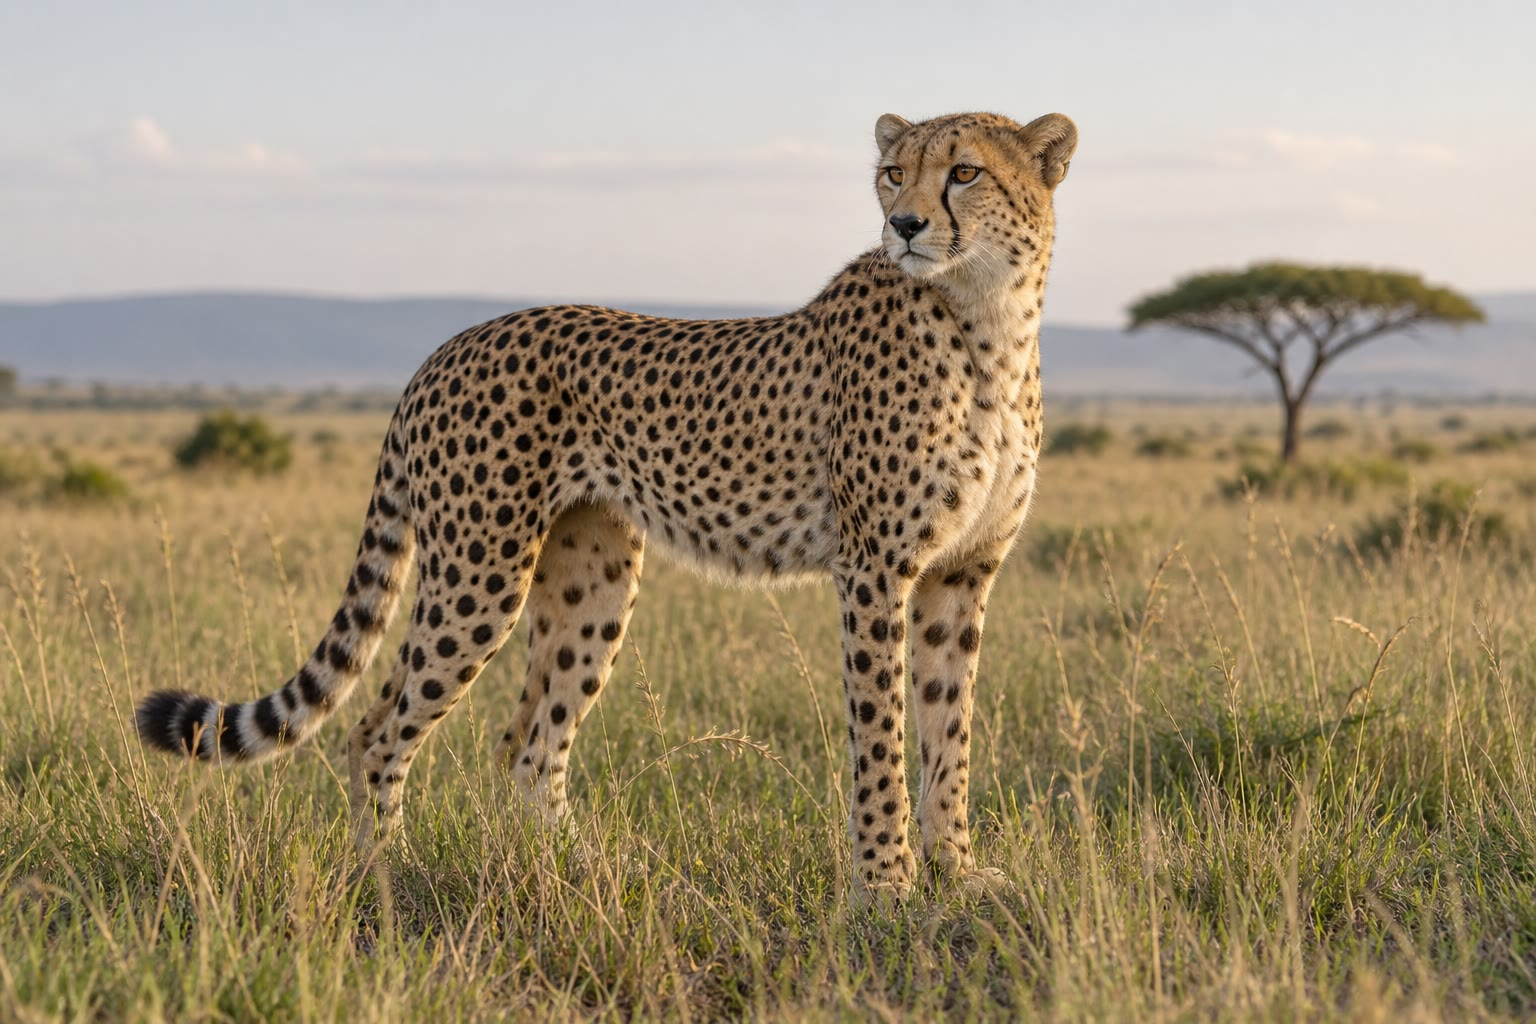
\includegraphics[width=0.52\linewidth]{images/book5/ai/b5-27-cheetah.jpg}

{\small बाएँ: मार्था, आख़िरी यात्री कबूतर, 1912 में सिनसिनाटी
चिड़ियाघर में खींची गई; उस जाति की संख्या जीवित स्मृति के भीतर अरबों में
थी (छायाचित्र एनो मायर द्वारा, सार्वजनिक डोमेन)। दाएँ: कोई चीता --- ऐसी
जाति जो कोई दस हज़ार वर्ष पहले किसी अड़चन से गुज़री और जिसके व्यष्टि
इतने एक-से हैं कि असंबंधित प्राणियों के बीच त्वचा-निरोप अस्वीकृत नहीं
होते।}
\end{omfigure}

\section{आवास: कितना, और किस आकार का}

\begin{proposition}[जातियाँ और क्षेत्रफल]\label{prop:b3:conservation-biology:area}
\index{जाति--क्षेत्रफल संबंध}\index{आवास विखंडन}\index{द्वीप जीवभूगोल}\index{गलियारा}\index{SLOSS बहस}\index{किनारा प्रभाव}
द्वीपों भर, और द्वीपों जैसा बरतने वाले आवास-खंडों भर, जातियों की संख्या
$S$ क्षेत्रफल $A$ के साथ किसी घात-नियम की तरह बढ़ती है,
\[
S = c\,A^{z}, \qquad z \approx 0.15\text{--}0.35,
\]
वही \emph{\omterm{prop:b3:conservation-biology:area}{जाति--क्षेत्रफल संबंध}} है (अरेनियस, 1921; मैकआर्थर तथा विल्सन
के \omterm{prop:b3:conservation-biology:area}{द्वीप जीवभूगोल} ने, 1967 में, उसकी व्याख्या आप्रवास तथा विलोपन के किसी
संतुलन के रूप में की, जिसमें विलोपन छोटे द्वीपों पर तेज़ होता है)।
$z = 0.25$ के साथ, किसी आवास के क्षेत्रफल का \qty{90}{\%} खोना अंततः
उसकी जातियों का $1 - 0.1^{0.25} = \qty{44}{\%}$ खो देता है; आधा खोना
\qty{16}{\%} खोता है। वह हानि तात्कालिक नहीं होती --- कोई
\emph{विलोपन-ऋण} दशकों भर चुकाया जाता है, ज्यों-ज्यों अपने खंडों के लिए
बहुत छोटी समष्टियाँ घटती जाएँ --- और किसी नियत क्षेत्रफल का टुकड़ों में
\emph{विखंडन} अपनी अलग हानियाँ जोड़ता है: हर खंड किसी छोटी समष्टि को
थामता है, \emph{\omterm{prop:b3:conservation-biology:area}{किनारा प्रभाव}} (हवा, गर्मी, परभक्षी, खरपतवार) वन में
सैकड़ों मीटर भीतर तक घुसते हैं, और जिन जातियों को भीतरी भाग चाहिए वे
क्षेत्रफल के हिसाब से अधिक खोती हैं। एक ही बड़ा अभयारण्य या उतने ही कुल
क्षेत्रफल के कई छोटे, इनमें से कौन अधिक जातियाँ बचाता है (यानी
\emph{SLOSS} बहस), यह जाति पर निर्भर करता है: बड़ा वाला बड़ी समष्टियाँ
तथा भीतरी आवास थामता है, छोटे वाले किसी महाविपदा का जोखिम बाँटते हैं और
अधिक आवास-प्रकारों का नमूना लेते हैं। खंडों को जोड़ने वाले
\emph{गलियारे} व्यष्टियों तथा जीनों को उनके बीच आने-जाने देते हैं, और
अलग-थलग समष्टियों को किसी अधिसमष्टि में बदल देते हैं जिसके भाग स्थानीय
विलोपन के बाद फिर बसाए जा सकते हैं और अंतःप्रजनन से उबारे जा सकते हैं
--- और इसीलिए अभयारण्यों के बीच की भूमि उतनी ही चिंता का विषय बन गई है
जितने अभयारण्य।
\end{proposition}
\begin{proof}
वह घात-नियम आनुभविक है, जो दुनिया भर के द्वीपसमूहों, झीलों,
पर्वत-शिखरों तथा वन-खंडों पर लघुगणक--लघुगणक अक्षों पर फिट किया गया है;
$z$ का मान किसी मुख्यभूमि के टुकड़ों के लिए कम (आप्रवास जातियों को
उपस्थित रखता है) और सच्चे द्वीपों के लिए अधिक होता है। आंशिक हानि सीधे
निकलती है: $S'/S = (A'/A)^{z}$। \omterm{prop:b3:conservation-biology:area}{द्वीप जीवभूगोल} की क्रियाविधि की जाँच
सिंबरलॉफ तथा विल्सन (1969) ने की, जिन्होंने फ़्लोरिडा के छोटे मैंग्रोव
टापुओं को धूमित किया, हर संधिपाद को मार डाला, और जातियों की संख्या को
वर्ष भर के भीतर अपने पिछले मानों पर लौटते देखा --- यानी कोई साम्य, पहले
से भिन्न जातियों के साथ: वह संख्या क्षेत्रफल तथा दूरी से तय होती है,
पहचानें संयोग से।
\end{proof}

\begin{omfigure}
\begin{tikzpicture}
\begin{loglogaxis}[
  width=0.6\linewidth, height=5.4cm,
  axis x line=bottom, axis y line=left,
  xmin=0.5, xmax=20000, ymin=5, ymax=300,
  xlabel={क्षेत्रफल (km$^2$)}, ylabel={जातियों की संख्या},
  xlabel style={font=\small, at={(axis description cs:0.5,-0.12)}, anchor=north}, ylabel style={font=\small},
  tick label style={font=\small}, xtick={1,10,100,1000,10000}, xticklabels={1,10,100,1000,10000}, ytick={10,30,100,300}, yticklabels={10,30,100,300},
  clip=false,
]
\addplot[very thick, omDef, domain=0.5:20000, samples=40] {20*x^0.25};
\addplot[only marks, mark=*, mark size=1.8pt, omDef!70!black] coordinates {(1,22) (3,24) (10,38) (30,44) (100,66) (300,80) (1000,110) (3000,150) (10000,190)};
\draw[dashed, gray] (axis cs:10000,5) -- (axis cs:10000,200) -- (axis cs:0.5,200);
\draw[dashed, gray] (axis cs:1000,5) -- (axis cs:1000,112.5) -- (axis cs:0.5,112.5);
\node[font=\scriptsize, omDef, anchor=south west] at (axis cs:1.2,215) {$S = c\,A^{0.25}$: लघुगणक अक्षों पर ढाल $z$};
\node[font=\scriptsize, anchor=west, align=left] at (axis cs:1200,40) {क्षेत्रफल का \qty{90}{\%} खोइए:\\जातियों का $0.1^{0.25} = \qty{56}{\%}$\\रखिए};
\end{loglogaxis}
\end{tikzpicture}

{\small लघुगणकीय अक्षों पर जाति--क्षेत्रफल नियम। उसकी ढाल वही घातांक $z$
है; उससे किसी सिकुड़े आवास से जातियों की अंततः होने वाली हानि पढ़ी जा
सकती है --- वन का दसवाँ भाग जातियों का लगभग आधा रखता है, न कि वह दसवाँ
भाग जो कोई रैखिक अनुमान देता।}
\end{omfigure}

\begin{omfigure}
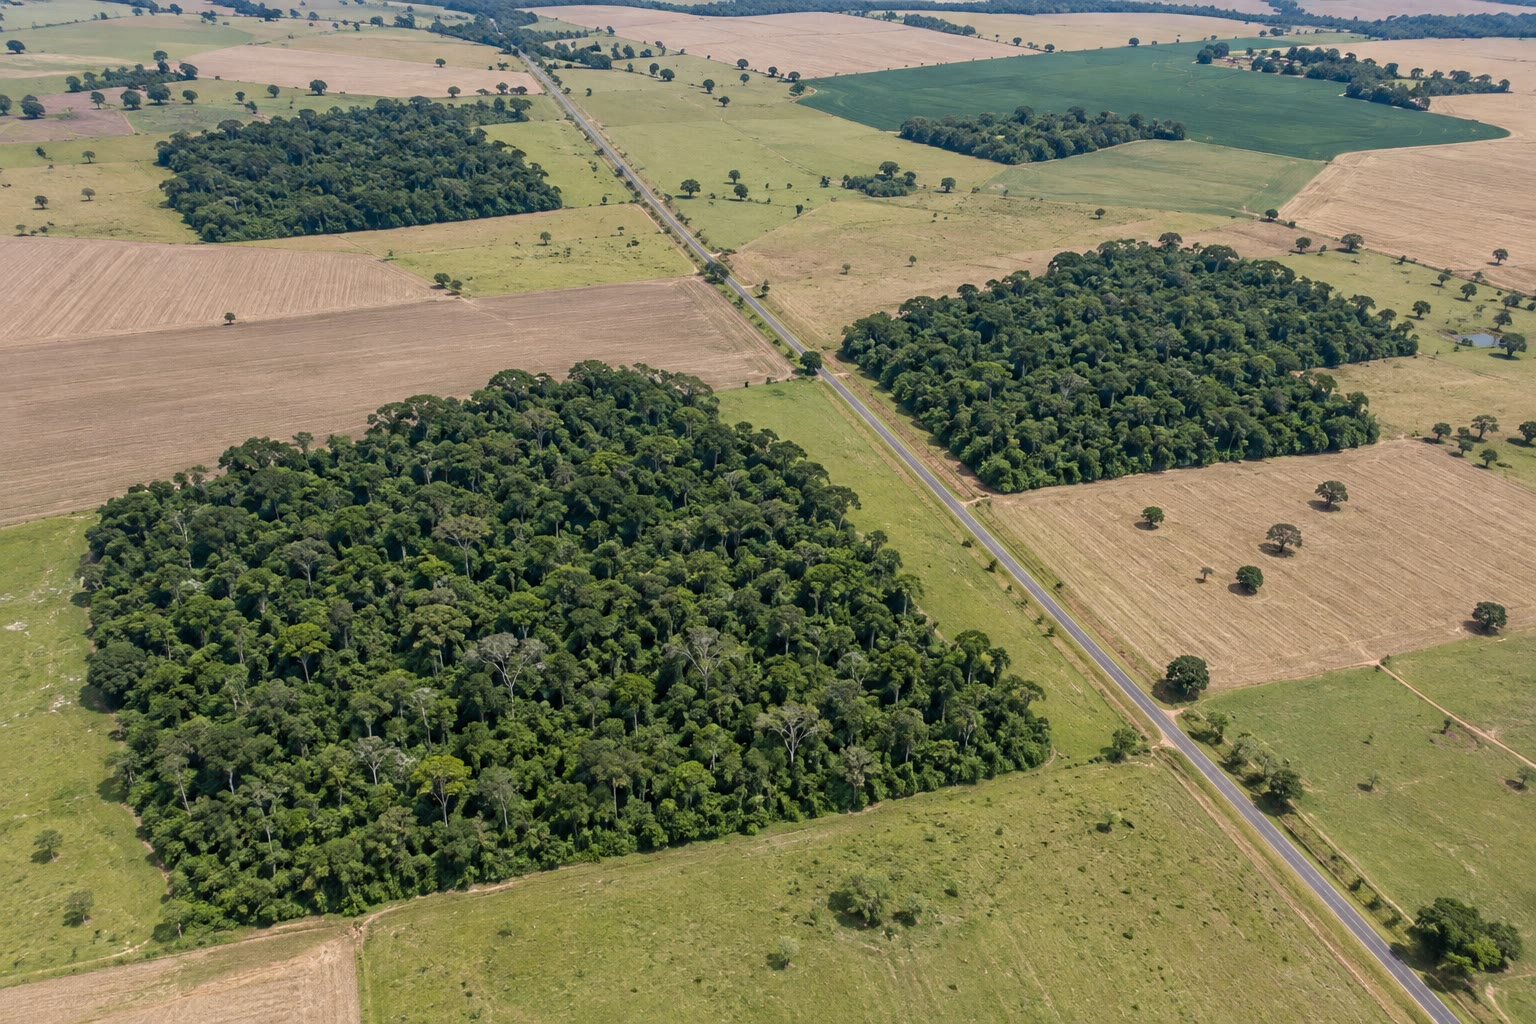
\includegraphics[width=0.6\linewidth]{images/book5/ai/b5-27-forest-fragments.jpg}

{\small खेतों के बीच वन-खंड, हवा से देखे गए: हर द्वीप उस समष्टि से छोटी
समष्टि थामता है जो पूरे वन ने थामी थी, ऐसे किसी क्षेत्र से किनारे तक
घिरा हुआ जिसे भीतरी जातियाँ काम में नहीं ले सकतीं, और ऐसे खेतों से अलग
किया गया जिन्हें वन-जातियाँ पार नहीं कर सकतीं।}
\end{omfigure}

\section{पूर्वानुमान और बचाव}

\begin{method}[समष्टि व्यवहार्यता विश्लेषण]\label{met:b3:conservation-biology:pva}
\index{समष्टि व्यवहार्यता विश्लेषण}\index{अर्ध-विलोपन}
किसी समष्टि के विलोपन के जोखिम का और उसे क्या घटाएगा उसका आकलन करने के
लिए: (1) उसकी गतिकी का कोई मॉडल बनाइए --- आयु- या अवस्था-विशिष्ट
उत्तरजीविता तथा जननक्षमता का कोई आव्यूह, जैसा वर्ष~2 के खंड की
जनसांख्यिकी में, जो कई वर्षों भर चिह्नित व्यष्टियों से आकलित हो; (2)
प्रसंभाव्यता जोड़िए --- जनसांख्यिकीय, हर व्यष्टि की नियति यादृच्छिक
खींचकर, और पर्यावरणीय, हर वर्ष की दरें उनके देखे गए प्रसरण से खींचकर,
बीच-बीच में महाविपदाओं के साथ; (3) जहाँ आँकड़े अनुमति दें वहाँ
घनत्व-निर्भरता तथा अंतःप्रजनन का आनुवंशिक ह्रास जोड़िए; (4) वर्तमान आकार
से रुचि के क्षितिज भर हज़ारों प्रक्षेप-पथों का अनुकरण कीजिए और वह अंश
दर्ज कीजिए जो किसी \emph{अर्ध-विलोपन} देहली से नीचे गिरे (यानी ऐसा आकार
जिससे वापसी असंभव मानी जाए); (5) निवेशों को बदलिए --- वयस्क उत्तरजीविता,
किशोर उत्तरजीविता, आवास क्षेत्रफल, दस प्राणियों का कोई स्थानांतरण --- और
देखिए कि कौन-सा बदलाव जोखिम सबसे अधिक घटाता है; प्रयास वहीं जाना चाहिए।
निर्गत कोई चौड़ी अनिश्चितता वाली प्रायिकता है, कोई भविष्यवाणी नहीं; उसका
मूल्य तुलनात्मक है, और उसने बार-बार दिखाया है कि दीर्घजीवी जातियों में
उत्तोलक वयस्क उत्तरजीविता है, जननक्षमता नहीं, और इसीलिए मछली-डोरियाँ उन
अल्बाट्रॉस समष्टियों को, जो हर दो वर्ष में एक अंडा देती हैं, घोंसलों की
किसी भी हानि से अधिक तेज़ी से मारती हैं।
\end{method}

\begin{proposition}[विलोपन तक का समय]\label{prop:b3:conservation-biology:time}
\index{विलोपन काल}
जिस समष्टि में उतार-चढ़ाव इसलिए हो कि पर्यावरण में होता है, जिसकी माध्य
वृद्धि-दर $\bar r$ शून्य के पास हो और वार्षिक वृद्धि-दर में प्रसरण
$\sigma^{2}$ हो, उसमें समष्टि-आकार का लघुगणक अपवाह सहित कोई यादृच्छिक
भ्रमण करता है, और आकार $N$ से विलोपन तक का प्रत्याशित समय केवल $N$ के
\emph{लघुगणक} की तरह बढ़ता है जब $\bar r < 0$ हो --- समष्टि दुगुनी करना
वर्षों की कोई नियत संख्या जोड़ता है --- और $N$ की किसी \emph{घात} की तरह
जब $\bar r > 0$ हो, जिसका घातांक $2\bar r/\sigma^{2} - 1$ है; अकेली
\omterm{def:b3:conservation-biology:small}{जनसांख्यिकीय प्रसंभाव्यता} के तहत वह $N$ के साथ \emph{चरघातांकी} रूप से
बढ़ता है, ताकि कोई समष्टि जो सौ पर जनसांख्यिकीय संयोग से सुरक्षित हो, दस
हज़ार पर भी पर्यावरणीय प्रसरण से खोई जा सकती है। व्यावहारिक परिणाम यह है
कि किसी समष्टि की वृद्धि का प्रसरण घटाना --- अधिक आवास, अधिक स्थलों तथा
चौड़े आहार से उसे बुरे वर्षों के सामने गद्दीदार बनाना --- उसके बने रहने
के लिए उसका माध्य बढ़ाने से अधिक कर सकता है।
\end{proposition}
\admitted

\begin{omfigure}
\begin{tikzpicture}
\begin{semilogyaxis}[
  width=0.62\linewidth, height=5.4cm,
  axis x line=bottom, axis y line=left,
  xmin=0, xmax=50, ymin=1, ymax=3000,
  xlabel={वर्ष}, ylabel={समष्टि आकार},
  xlabel style={font=\small, at={(axis description cs:0.5,-0.12)}, anchor=north}, ylabel style={font=\small},
  tick label style={font=\small}, xtick={0,10,20,30,40,50}, ytick={1,10,100,1000}, yticklabels={1,10,100,1000},
  clip=false,
]
\addplot[thick, omDef] coordinates {(0,200) (2,240) (4,190) (6,260) (8,300) (10,220) (12,180) (14,250) (16,330) (18,280) (20,350) (22,300) (24,260) (26,340) (28,420) (30,380) (32,450) (34,400) (36,520) (38,480) (40,560) (42,500) (44,600) (46,650) (48,610) (50,700)};
\addplot[thick, omThm] coordinates {(0,200) (2,150) (4,180) (6,120) (8,90) (10,110) (12,70) (14,50) (16,60) (18,35) (20,40) (22,25) (24,18) (26,22) (28,12) (30,8) (32,9) (34,5) (36,3) (38,2) (40,1)};
\addplot[thick, omMeth!70!black] coordinates {(0,200) (2,210) (4,170) (6,200) (8,140) (10,160) (12,120) (14,140) (16,90) (18,110) (20,80) (22,95) (24,60) (26,75) (28,50) (30,55) (32,40) (34,45) (36,30) (38,35) (40,28) (42,30) (44,22) (46,25) (48,20) (50,22)};
\draw[dashed, gray] (axis cs:0,20) -- (axis cs:50,20); \node[font=\scriptsize, gray, anchor=north east] at (axis cs:49,18) {अर्ध-विलोपन देहली};
\node[font=\scriptsize, omDef, anchor=west] at (axis cs:50.5,700) {$\bar r > 0$: बना रहता है};
\node[font=\scriptsize, omMeth!70!black, anchor=west] at (axis cs:50.5,22) {$\bar r \approx 0$: नीचे बहता};
\node[font=\scriptsize, omThm, anchor=west] at (axis cs:40.5,1.3) {$\bar r < 0$: 40 वर्षों में गया};
\end{semilogyaxis}
\end{tikzpicture}

{\small उन्हीं दो सौ प्राणियों से तीन अनुकरित प्रक्षेप-पथ, जो केवल माध्य
वृद्धि-दर में भिन्न हैं; कोई व्यवहार्यता विश्लेषण इनके हज़ारों चलाता है
और गिनता है कि कितने उस देहली को पार करते हैं। वर्ष-दर-वर्ष का प्रसरण ही
बीच वाले मामले को भी कोई जुआ बनाता है।}
\end{omfigure}

\begin{definition}[औज़ार]\label{def:b3:conservation-biology:tools}
\index{IUCN लाल सूची}\index{आक्रामक जाति}\index{बहिःस्थाने संरक्षण}\index{बंदी प्रजनन}\index{पुनःस्थापन}\index{पुनर्वन्यीकरण}\index{पोषी अनुप्रपात}
\emph{IUCN लाल सूची} जातियों को मात्रात्मक कसौटियों से वर्गीकृत करती है:
दस वर्षों या तीन पीढ़ियों भर \qty{30}{\%}, \qty{50}{\%} या \qty{80}{\%}
का ह्रास, \qty{20000}{}, \qty{5000}{} या \qty{100}{km^2} से नीचे का
विस्तार, \qty{10000}{}, \qty{2500}{} या \qty{250}{} परिपक्व व्यष्टियों
से नीचे की कोई समष्टि, या कोई मॉडल की गई विलोपन प्रायिकता किसी जाति को
संकटप्राय, संकटग्रस्त या अतिसंकटग्रस्त ठहराती है; स्तनधारियों का चौथाई
और पक्षियों का आठवाँ भाग इस पर खरा उतरता है। कारण पहले आवास-हानि हैं,
फिर अति-कटाई, \emph{आक्रामक जातियाँ} (ऐसे द्वीपों पर ले जाए गए परभक्षी
तथा प्रतिस्पर्धी जिनकी जातियाँ उनसे कभी मिली ही न थीं: चूहों, बिल्लियों
तथा स्टोटों ने न्यूज़ीलैंड के अधिकांश पक्षी ले लिए हैं, और अकेली किसी
भूरे वृक्ष-सर्प जाति ने गुआम के अधिकांश), प्रदूषण तथा जलवायु परिवर्तन।
प्रतिक्रियाएँ: भूमि के छठे भाग को ढकते संरक्षित क्षेत्र; आक्रमणकारियों
का नियंत्रण या उन्मूलन (डेढ़ सौ द्वीप चूहों से ख़ाली किए गए);
\emph{बहिःस्थाने} संरक्षण --- आर्कटिक स्थायी तुषार में किसी तहख़ाने में
दस लाख नमूने रखते बीज-कोष, जमे हुए भ्रूण, और वंशावलियों को बंधुत्व
न्यूनतम करने के लिए सँभालते हुए \emph{बंदी प्रजनन}, जो कैलिफ़ोर्निया
कॉन्डोर को 1987 के बाईस पक्षियों से और काले-पैर वाले फेरेट को अठारह से
वापस लाया; \emph{पुनःस्थापन}, जो लगभग तिहाई बार सफल होता है और तब अधिक
जब मूल हानि का कारण हटा दिया गया हो; और \emph{पुनर्वन्यीकरण}, यानी बड़े
प्राणियों तथा उनसे चलने वाली प्रक्रियाओं की वापसी --- येलोस्टोन के
भेड़िये, जिनके परभक्षण ने और उसके डर ने एल्क को नदी-तटों से हटा दिया और
विलो, ऐस्पन, बीवर तथा गीतपक्षियों को लौटने दिया, यानी कोई \emph{पोषी
अनुप्रपात} जो किसी मांसाहारी से किसी नदी के आकार तक चलता है।
\end{definition}

\begin{omfigure}
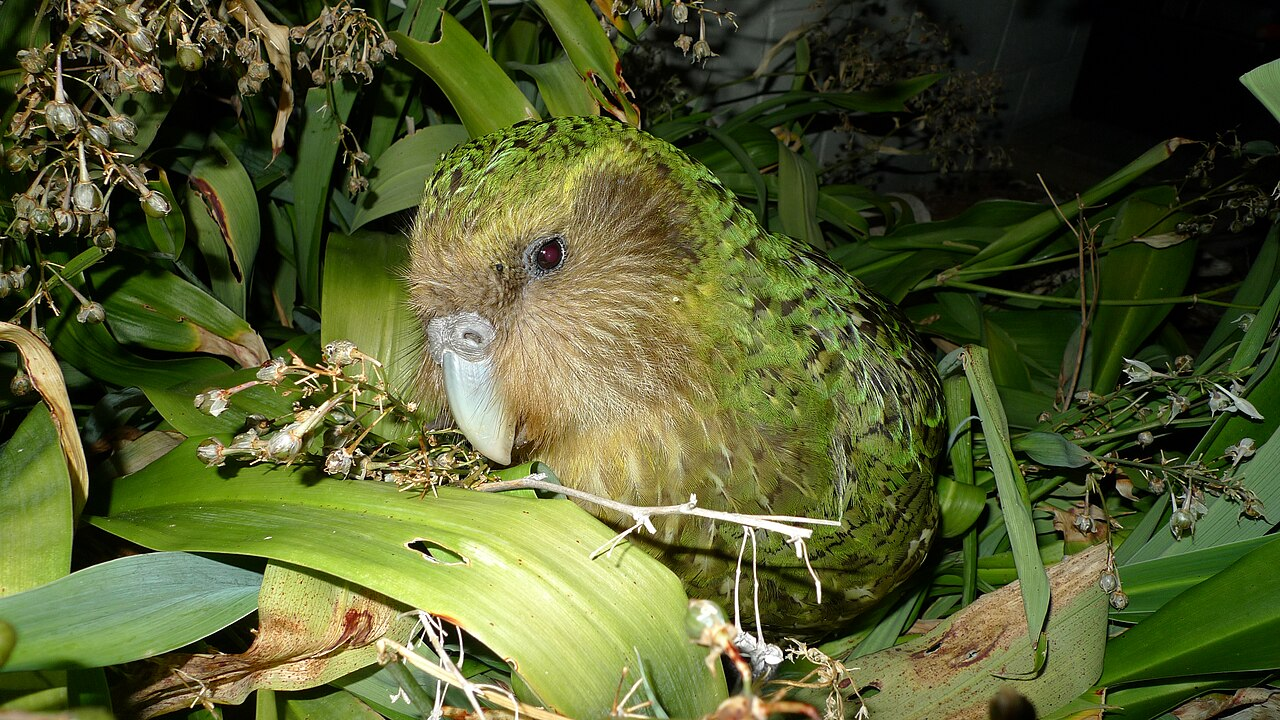
\includegraphics[width=0.46\linewidth]{images/book5/kakapo-sirocco.jpg}\hspace{0.04\linewidth}
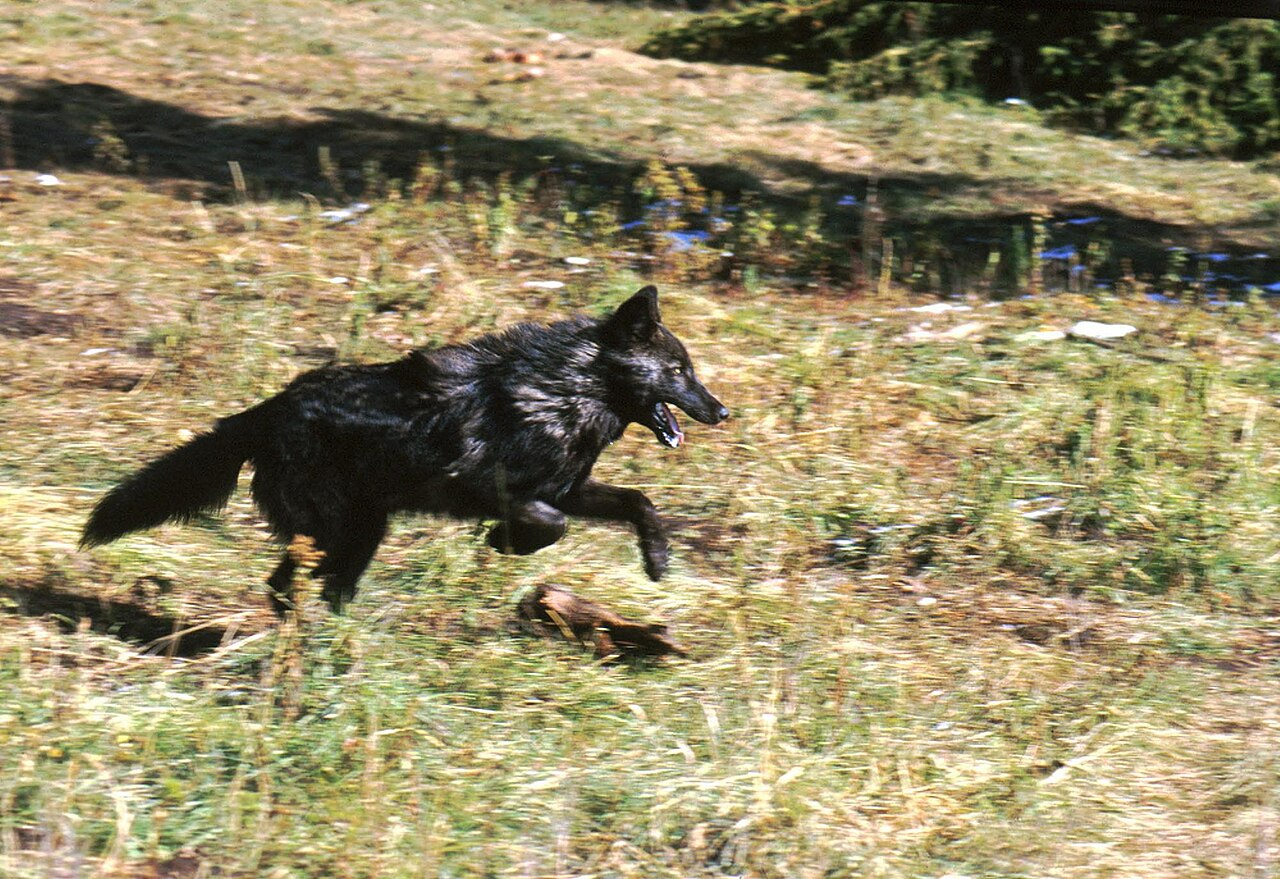
\includegraphics[width=0.46\linewidth]{images/book5/yellowstone-wolves-1996.jpg}

{\small बाएँ: सिरोको, कोई काकापो --- 1995 के इक्यावन बचे हुओं में से एक,
अब कोई ढाई सौ में से एक, जिनमें से हर एक का नाम है और जो परभक्षी-मुक्त
द्वीपों पर निगरानी में हैं (छायाचित्र: संरक्षण विभाग, न्यूज़ीलैंड, CC BY
2.0)। दाएँ: 1996 में येलोस्टोन के भेड़िये, उनके \omterm{def:b3:conservation-biology:tools}{पुनःस्थापन} के बाद की
पहली सर्दी (छायाचित्र: राष्ट्रीय उद्यान सेवा, सार्वजनिक डोमेन)।}
\end{omfigure}

\begin{example}[तीन वापसियाँ]\label{ex:b3:conservation-biology:recoveries}
काकापो: 1995 में इक्यावन पक्षी, सब परभक्षियों से ख़ाली किए गए द्वीपों पर
ले जाए गए; हर पक्षी कोई प्रेषित्र पहनता है, हर घोंसला कैमरे से देखा जाता
है, माँ के चूकने पर चूज़े हाथ से पाले जाते हैं, जिन वर्षों रिमू वृक्ष
फलते हैं उन वर्षों नरों को खिलाकर प्रजनन-दशा में लाया जाता है, और
वंशावली इस तरह सँभाली जाती है कि आख़िरी फियोर्डलैंड नर के दुर्लभ जीन
समष्टि में बने रहें; हर काकापो का जीनोम अनुक्रमित किया जा चुका है। अब
ढाई सौ, और कोई $N_{e}$ जिसे जीनोम सौ के पास रखते हैं। हूपिंग सारस: 1941
में पंद्रह पक्षी, कोई एक ही प्रवासी झुंड, जंगली घोंसलों से लिए गए अंडों
से बंदी अवस्था में प्रजनित, अतिलघु विमानों के पीछे नए प्रवास-मार्ग सिखाए
गए, और अब कोई आठ सौ। हंपबैक व्हेल: कुछ हज़ार तक शिकार की गई, 1966 में
संरक्षित, और अब एक लाख से पार, यानी प्रति वर्ष लगभग \qty{8}{\%} की
वृद्धि, जो दिखाती है कि जब किसी दीर्घजीवी प्राणी के ह्रास का इकलौता कारण
हटा दिया जाए तब वह क्या करता है। हर वापसी की लागत करोड़ों डॉलर और दशक
रही; अध्याय का अंकगणित बताता है कि वह प्रयास संख्याओं के भँवर तक पहुँचने
से पहले क्यों करना पड़ा, और वह बाद की किसी भी बचाव-कार्रवाई से सस्ता
क्यों रहा।
\end{example}

\begin{omfigure}
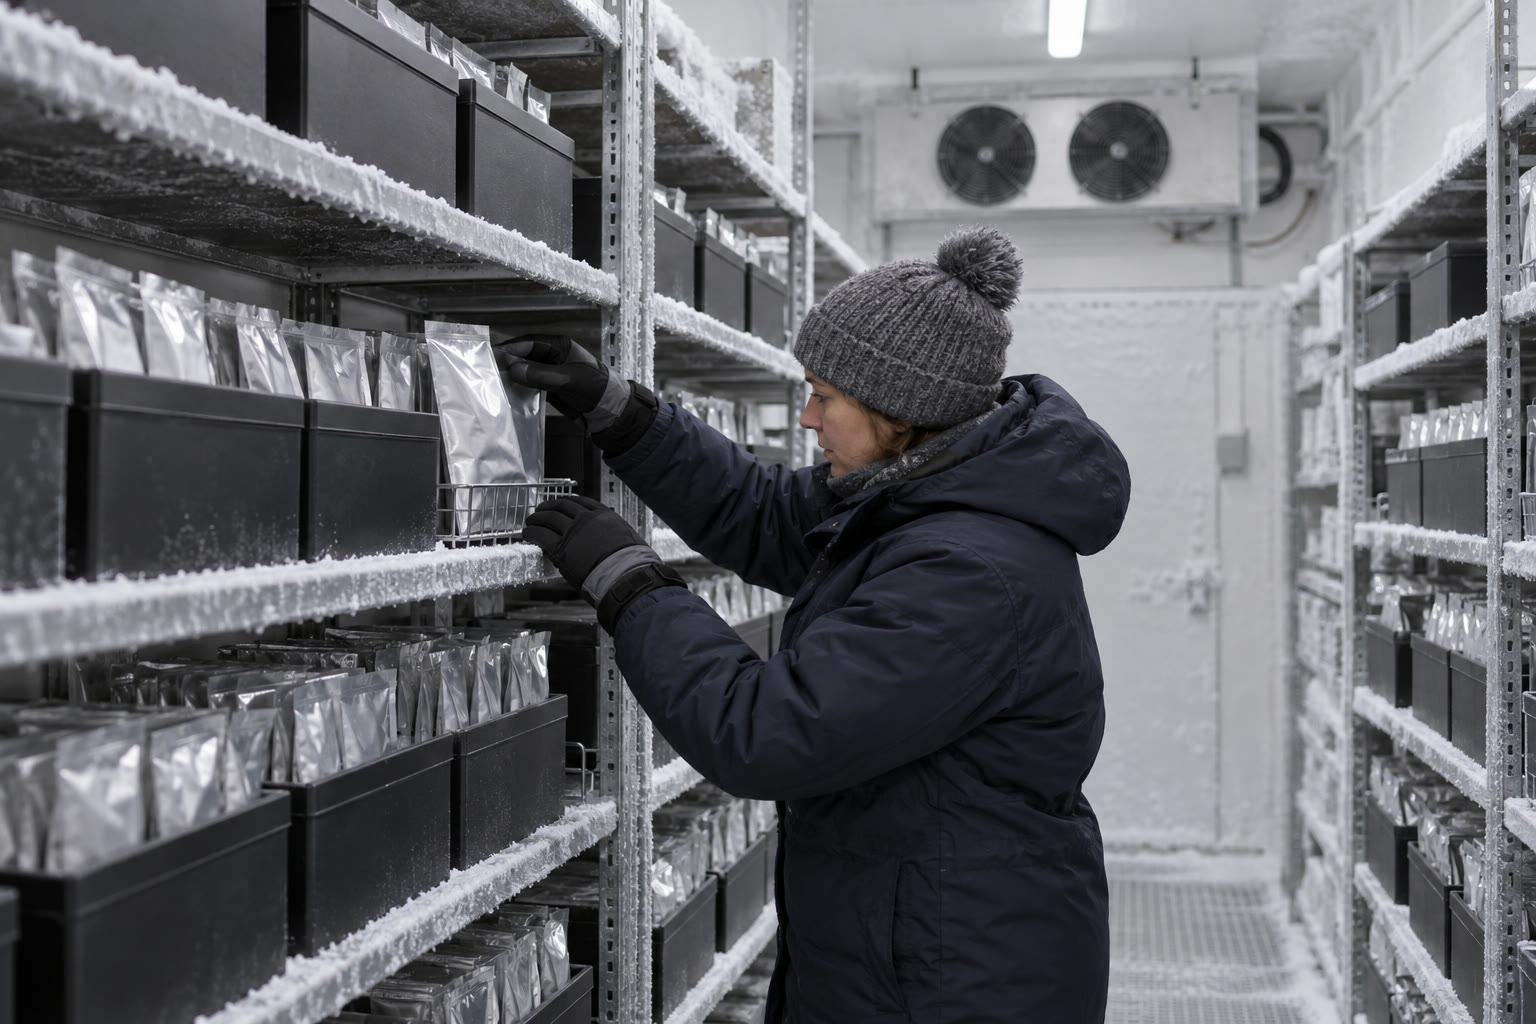
\includegraphics[width=0.56\linewidth]{images/book5/ai/b5-27-seed-vault.jpg}

{\small स्थायी तुषार में कोई बीज-तहख़ाना: दस लाख फ़सली तथा वन्य-पादप
नमूनों की प्रतिलिपियाँ, जिन संग्रहों से वे आईं उनकी हानि के विरुद्ध
\qty{-18}{\celsius} पर रखी गईं --- यानी बीमे की तरह संरक्षण, किसी जाति
के जीनोम के पैमाने पर।}
\end{omfigure}

\begin{remark}[रखने का अंकगणित]\label{rem:b3:conservation-biology:remark}
इस पाठ्यक्रम का हर अध्याय किसी संख्या पर समाप्त हुआ है, और यह कई पर
समाप्त होता है: कोई प्रभावी आकार, प्रति पीढ़ी $1/2N_{e}$ से बढ़ता कोई
\omterm{thm:b3:conservation-biology:ne}{अंतःप्रजनन गुणांक}, कोई घातांक $z$ जो खोए हेक्टेयरों को खोई जातियों में
बदल देता है, किसी शताब्दी भर विलोपन की कोई प्रायिकता। वे कच्ची हैं ---
गणना अनिश्चित है, प्रसरण का अनुमान लगाया गया है, मॉडल कोई व्यंग्यचित्र
है --- और वही हैं जो लुप्त होते पक्षियों के बारे में किसी भावना को इस
निर्णय में बदलती हैं कि कौन-से पचास हेक्टेयर ख़रीदे जाएँ और कौन-से आठ
प्राणी हटाए जाएँ। यह जीवविज्ञान वही जीवविज्ञान है जो बाक़ी पुस्तक का है:
अपवाह, वरण, जनसांख्यिकी, व्यवहार, किसी समष्टि की अपने आवास पर और किसी
आवास की अपनी समष्टियों पर निर्भरता। नया केवल वह तात्कालिकता है, और यह
तथ्य कि वह प्रयोग एक ही बार चलाया जा रहा है, बिना किसी नियंत्रण के, उन
जातियों पर जो बची हैं।
\end{remark}

\section{अभ्यास}

\begin{exercise}[$\star$]\label{exo:b3:conservation-biology:1}
\omterm{def:b3:conservation-biology:small}{जनसांख्यिकीय प्रसंभाव्यता}, \omterm{def:b3:conservation-biology:small}{पर्यावरणीय प्रसंभाव्यता} तथा \omterm{def:b3:conservation-biology:small}{ऐली प्रभाव}
परिभाषित कीजिए, और अध्याय से हर एक का एक उदाहरण दीजिए।
\end{exercise}

\begin{exercise}[$\star$]\label{exo:b3:conservation-biology:2}
\omterm{thm:b3:conservation-biology:ne}{प्रभावी समष्टि आकार} क्या है, और किसी असली समष्टि की तीन ऐसी विशेषताएँ
बताइए जो उसे गणना से छोटा बनाती हैं।
\end{exercise}

\begin{exercise}[$\star$]\label{exo:b3:conservation-biology:3}
जाति--क्षेत्रफल नियम बताइए। यदि $z = 0.25$ हो, तो अपना आधा क्षेत्रफल
खोने के बाद कोई आवास जातियों का कितना अंश रखता है? नौ-दसवाँ भाग खोने के
बाद? निन्यानबे-सौवाँ भाग खोने के बाद?
\end{exercise}

\begin{exercise}[$\star$]\label{exo:b3:conservation-biology:4}
50/500 नियम समझाइए, और यह भी कि हर संख्या किससे बचाती है।
\end{exercise}

\begin{exercise}[$\star\star$]\label{exo:b3:conservation-biology:5}
200 हाथी-सीलों के किसी झुंड में 8 प्रजननशील नर और 120 प्रजननशील मादाएँ
हैं। $N_{e}$ तथा प्रति पीढ़ी विषमयुग्मजता की हानि निकालिए। उसका चौथाई
खोने में कितनी पीढ़ियाँ?
\end{exercise}

\begin{exercise}[$\star\star$]\label{exo:b3:conservation-biology:6}
किसी समष्टि की संख्या लगातार पाँच पीढ़ियों में 1000, 1000, 20, 1000,
1000 रही। उस अवधि भर $N_{e}$ तथा बची हुई विषमयुग्मजता निकालिए, और अचल
1000 से तुलना कीजिए।
\end{exercise}

\begin{exercise}[$\star\star$]\label{exo:b3:conservation-biology:7}
$N_{e} \approx 10$ वाले पच्चीस फ़्लोरिडा पैंथर: 5 पीढ़ियों में जुड़ा
अंतःप्रजनन? यदि $F$ के हर \qty{10}{\%} पर सुयोग्यता \qty{5}{\%} गिरती हो,
तो सुयोग्यता कितनी गिरी है? आठ असंबंधित मादाएँ जोड़ना अगली पीढ़ी में $F$ का
क्या करता है?
\end{exercise}

\begin{exercise}[$\star\star$]\label{exo:b3:conservation-biology:8}
येलोस्टोन: 1995--96 में 31 भेड़िये छोड़े गए, 2003 तक उद्यान में लगभग
100। $r$ का आकलन कीजिए; यदि वृद्धि चलती रहती तो 2020 में कितने होते, और
वह चली क्यों नहीं?
\end{exercise}

\begin{exercise}[$\star\star$]\label{exo:b3:conservation-biology:9}
अध्याय की IUCN कसौटियों से वर्गीकरण कीजिए: (a) कोई मेंढक जिसकी समष्टि दस
वर्षों में \qty{60}{\%} गिरी; (b) 180 परिपक्व व्यष्टियों का कोई पादप;
(c) कोई मछली जिसका विस्तार \qty{3000}{km^2} है; (d) \num{30000}
व्यष्टियों का कोई पक्षी जो प्रति दशक \qty{10}{\%} घट रहा है।
\end{exercise}

\begin{exercise}[$\star\star\star$]\label{exo:b3:conservation-biology:10}
$N$ युग्मों की कोई समष्टि, जिसमें हर युग्म $1/2$ प्रायिकता से दो जीवित
संतानें देता है और अन्यथा कोई नहीं (\omterm{def:b3:conservation-biology:small}{जनसांख्यिकीय प्रसंभाव्यता})।
$N = 2$, $5$, $10$, $20$ के लिए वह प्रायिकता निकालिए कि पूरी समष्टि एक
ही पीढ़ी में चूक जाए, और टिप्पणी कीजिए कि जनसांख्यिकीय जोखिम $N$ के साथ
कैसे बदलता है।
\end{exercise}

\begin{exercise}[$\star\star\star$]\label{exo:b3:conservation-biology:11}
$z = 0.25$ के साथ जाति--क्षेत्रफल नियम, और कोई वन जो 10 बराबर अलग-थलग
खंडों में काटा गया। किसी एक खंड में प्रत्याशित जातियों की तुलना मूल के
दसवें भाग से कीजिए, और तर्क दीजिए कि खंडों भर का कुल यों ही मूल क्यों
नहीं है --- क्या तय करता है कि सब खंड मिलकर पूरे वन से अधिक जातियाँ
थामते हैं या कम?
\end{exercise}

\begin{exercise}[$\star\star\star$]\label{exo:b3:conservation-biology:12}
प्रति पीढ़ी कुछ प्रवासी जोड़ना ($m N_{e} \approx 1$) किसी छोटी समष्टि
में विविधता की हानि को अधिकांशतः क्यों रोक देता है, और स्थानीय अनुकूलन
में उसकी क्या लागत है? तर्क के लिए अपवाह, $1/2N_{e}$, तथा प्रवासियों से
बदले गए युग्मविकल्पियों के अंश, $m$, के बीच के संतुलन का उपयोग कीजिए।
\end{exercise}

\section{समस्या: पचास और पाँच सौ}

\begin{problem}[{सप्तांत समस्या --- संख्याओं में कोई वापसी-कार्यक्रम:
किसी उबारी गई तोता-समष्टि का प्रभावी आकार तथा उसका अंतःप्रजनन, कोई
आनुवंशिक बचाव, कोई सिकुड़ता वन जितनी जातियाँ रखेगा, पुनःस्थापित भेड़ियों
की वृद्धि, और वे श्रेणियाँ तथा लागतें, जो $N_{e}$, दस पीढ़ियों बाद के
अंतःप्रजनन और रखी गई जातियों के अंश पर समाप्त होती हैं}]
\label{pb:b3:conservation-biology:1}
आँकड़े: 60 वयस्कों की कोई तोता-समष्टि, 20 नर और 40 मादाएँ, सब
प्रजननशील; पीढ़ी-काल \qty{10}{yr}। पिछली पाँच पीढ़ियों भर समष्टि का
इतिहास: 500, 100, 60, 51, 60। अंतःप्रजनन अवसाद: $F$ के हर \qty{0.1}{} पर
सुयोग्यता \qty{6}{\%} गिरती है। बचाव: 60 में 10 असंबंधित पक्षी जोड़े गए।
वन: \qty{2000}{km^2} घटकर \qty{300}{km^2}, $z = 0.25$; जातियाँ अब 180।
भेड़िये: 31 छोड़े गए, 8 वर्ष बाद 100, उद्यान में धारण क्षमता लगभग 120।
लागत: तोतों के लिए प्रति वर्ष चालीस लाख डॉलर।

\medskip
\noindent\textbf{भाग I --- प्रभावी आकार।}
\begin{enumerate}
  \item वर्तमान 60 के \omterm{thm:b3:conservation-biology:ne}{लिंग अनुपात} से $N_{e}$। गणना से तुलना कीजिए।
  \item इतिहास की पाँच पीढ़ियों भर हरात्मक-माध्य $N_{e}$। कौन-सी पीढ़ी
        हावी है?
  \item हरात्मक-माध्य $N_{e}$ का उपयोग करते हुए, उन पाँच पीढ़ियों भर
        जुड़ा अंतःप्रजनन (यथार्थ सूत्र तथा रैखिक सन्निकटन)।
  \item उस अंतःप्रजनन से खोई सुयोग्यता।
  \item पाँच पीढ़ियों बाद बची विषमयुग्मजता, मूल के किसी अंश के रूप में।
  \item यदि समष्टि अब वर्तमान \omterm{thm:b3:conservation-biology:ne}{लिंग अनुपात} के साथ 60 पर रखी जाए, तो दस और
        पीढ़ियों में वह किस $F$ तक पहुँचेगी, और कितनी सुयोग्यता-हानि? वह
        कितने वर्ष हैं?
\end{enumerate}

\medskip
\noindent\textbf{भाग II --- बचाव।}
\begin{enumerate}[resume]
  \item दस असंबंधित पक्षी उन 60 में मिलते हैं। अगली पीढ़ी में
        नवागंतुकों से आने वाले युग्मविकल्पियों का अंश लगभग $10/70$ है;
        एक देशज तथा एक नवागंतुक जनक वाली संतानों का \omterm{thm:b3:conservation-biology:ne}{अंतःप्रजनन गुणांक}
        $0$ है। यदि संगम यादृच्छिक हो तो अगली पीढ़ी में समष्टि का माध्य
        $F$ आकलित कीजिए।
  \item समझाइए कि $F$ तुरंत क्यों गिरता है पर विषमयुग्मजता केवल
        तब-तब बढ़ती है जब प्रवासियों के युग्मविकल्पी फैलें, और दूसरे
        बचाव की ज़रूरत क्यों पड़ सकती है।
  \item बराबर \omterm{thm:b3:conservation-biology:ne}{लिंग अनुपात} के साथ $N_{e} = 500$ तक पहुँचने के लिए कितने
        वयस्क चाहिए? 70 पक्षियों से $r = \qty{0.05}{yr^{-1}}$ पर, कितने
        वर्ष?
  \item वह कार्यक्रम कमज़ोर माताओं से अंडे हाथ से पालने के लिए हटाता है,
        जिससे प्रति युग्म पंख निकले चूज़ों की माध्य संख्या बढ़ती है पर
        कुल-आकार बराबर हो जाते हैं। कुल-आकार बराबर करना $N_{e}$ को गणना
        से ऊपर ($2N$ की ओर) क्यों \emph{उठाता} है?
  \item किसी अलग दक्षिणी वंशक्रम का आख़िरी नर जंगल में बंध्य है। दो
        हस्तक्षेप और जीन-कोश के लिए उनकी लागतें सुझाइए।
  \item $N_{e} = 500$ तक पहुँचने के 40 वर्षों भर प्रति वर्ष चालीस लाख
        डॉलर पर, कुल लागत, और प्रति जोड़े गए पक्षी की लागत। क्या वह
        महँगा है? किसके सामने?
\end{enumerate}

\medskip
\noindent\textbf{भाग III --- वन।}
\begin{enumerate}[resume]
  \item \qty{300}{km^2} पर वह वन जातियों का कितना अंश रखेगा; जातियों की
        प्रत्याशित संख्या, और विलोपन-ऋण (अभी उपस्थित वे जातियाँ जो खो
        जाएँगी)।
  \item यदि इसके बजाय वे \qty{300}{km^2} \qty{100}{km^2} के तीन
        अलग-थलग खंड होते, तो प्रति खंड जातियाँ; यदि खंड पूरी तरह भिन्न
        जातियाँ थामें तो कुल; यदि एक-सी थामें तो कुल। क्या तय करता है?
  \item \qty{20}{km^2} का कोई गलियारा उन तीन खंडों को जोड़ता है। उन्हें
        \qty{320}{km^2} का एक ही क्षेत्रफल मानिए: प्रत्याशित जातियाँ।
        प्रश्न~14 के एक-सी-जातियों वाले मामले से तुलना कीजिए।
  \item उस वन के सबसे बड़े परभक्षी को बने रहने के लिए प्रति युग्म
        \qty{50}{km^2} और 50 का कोई $N_{e}$ चाहिए। क्या पूरा
        \qty{300}{km^2} उसे थाम सकता है? क्या कोई खंड? कसौटी के रूप में
        क्षेत्रफल बनाम जातियों की संख्या के बारे में यह क्या कहता है?
  \item आकलन कीजिए कि विलोपन-ऋण चुकाने में कितना समय लगता है, यदि खोई
        जाने वाली जातियों की समष्टियाँ 200 से 10 की किसी अर्ध-विलोपन
        देहली तक प्रति वर्ष \qty{3}{\%} की दर से घट रही हों।
  \item जब विखंडन \omterm{prop:b3:conservation-biology:area}{किनारा प्रभाव} जोड़ता है तब जाति--क्षेत्रफल नियम हानि
        को कम क्यों आँकता है, और जब आसपास की भूमि आंशिक रूप से काम की हो
        तब अधिक क्यों?
\end{enumerate}

\medskip
\noindent\textbf{भाग IV --- भेड़िये और सूचियाँ।}
\begin{enumerate}[resume]
  \item भेड़िये: $r$, जो 8 वर्षों में $31 \to 100$ से निकले, और दुगुना
        होने का समय।
  \item $K = 120$ की ओर संभार्य वृद्धि: चरघातांकी के बजाय संभार्य वृद्धि
        के तहत, प्रश्न~19 के $r$ के साथ 31 से शुरू करके 8 वर्षों बाद
        समष्टि ($N(t) = K/[1 + (K/N_{0} -
        1)\mathrm{e}^{-rt}]$ का उपयोग कीजिए)। देखे गए 100 से कौन बेहतर
        बैठता है, और वह पहले वर्षों में घनत्व-निर्भरता के बारे में क्या
        कहता है?
  \item एल्क 1995 में \num{17000} थे और 2015 में \num{4000}। ह्रास की
        औसत वार्षिक दर। 100 भेड़ियों पर, हर एक प्रति वर्ष \num{20} एल्क
        खाते हुए, भेड़िये उसमें से कितना समझा सकते हैं?
  \item तोते (60 परिपक्व व्यष्टि) और बचाव-पूर्व वन-परभक्षी का IUCN
        कसौटियों से वर्गीकरण कीजिए।
  \item यात्री कबूतर: 1800 में पाँच अरब, 1914 में विलुप्त। यदि वह ह्रास
        1870 से, जब अब भी अरबों थे, 1914 के एक पक्षी तक चरघातांकी रहा
        हो, तो वह किस वार्षिक दर का संकेत देता है? \omterm{def:b3:conservation-biology:small}{ऐली प्रभाव} आख़िरी
        दशकों को चरघातांकी से तेज़ क्यों बना देता है?
  \item किसी अनुच्छेद में समझाइए कि कोई PVA 1850 में यात्री कबूतर को
        सुरक्षित क्यों बताता, और वह क्या चूक जाता।
  \item संक्षेप में: वर्तमान $N_{e}$ (प्रश्न~1), 60 पर दस और पीढ़ियों बाद
        $F$ (प्रश्न~6), और सिकुड़ा हुआ वन जातियों का जो अंश रखता है
        (प्रश्न~13)।
\end{enumerate}
\end{problem}
